\section{Medición del Entrainment}
\label{sec:method_entrainment}

\begin{figure}
\centering
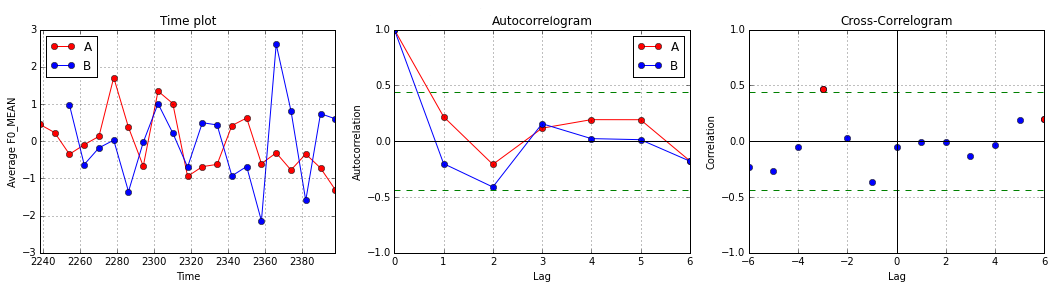
\includegraphics[width=15cm]{images/time_plot_with_cross_correlation.png}
\caption{Time-plot generado por el método TAMA, junto a su autocorrelograma y correlograma cruzado}
\label{fig:time_plot_with_bivariate}
\end{figure}

Considerando todo lo mencionado en la sección \ref{sec:analisis_bivariado}, procedimos a definir una medida de \entrainment basándonos en el cálculo de la correlación cruzada muestral. Recordemos que, bajo la definición dada en la ecuación \ref{cross_correlation_definition} de $r_{AB}(k)$, al tomar $k \geq 0$ medíamos cuánto influía $B$ sobre los futuros valores de $A$, y viceversa cuando $k \leq 0$.

Con esto en mente, definimos $\fwentrainment{AB}$ como el valor de $r_{AB}(k)$ con mayor valor absoluto, dado $k \leq 0$. Análogamente lo definimos para $\fwentrainment{BA}$. En \ref{fig:time_plot_with_bivariate} podemos observar en el lag -3 y 6 los valores de \entrainment elegidos del correlograma.

Por último, cabe mencionar que a diferencia de \cite{KOU2008.2} dónde sólo se hacía un análisis de significancia, nosotros vamos a utilizar esta medida independientemente de si es o no estadísticamente diferente de cero.
